\documentclass[11pt,a4paper]{article}

\usepackage[margin=1in]{geometry}
\usepackage{graphicx}
\usepackage{booktabs}
\usepackage{array}
\usepackage{longtable}
\usepackage{caption}
\usepackage{subcaption}
\usepackage{xcolor}
\usepackage{listings}
\usepackage{amsmath}
\usepackage{amssymb}
\usepackage{enumitem}
\usepackage{fancyhdr}
\usepackage{titlesec}
\usepackage[hidelinks]{hyperref}

\definecolor{codebg}{RGB}{245,245,245}
\definecolor{codekw}{RGB}{0,80,150}
\definecolor{codecomment}{RGB}{110,110,110}
\definecolor{codestring}{RGB}{140,20,20}

\lstset{
  backgroundcolor=\color{codebg},
  basicstyle=\ttfamily\small,
  keywordstyle=\color{codekw}\bfseries,
  commentstyle=\color{codecomment}\itshape,
  stringstyle=\color{codestring},
  showstringspaces=false,
  breaklines=true,
  frame=single,
  rulecolor=\color{gray!40},
  numbers=left,
  numberstyle=\tiny\color{gray},
  xleftmargin=1.8em,
  language=Python
}

\titleformat{\section}{\normalfont\Large\bfseries}{\thesection}{1em}{}
\titleformat{\subsection}{\normalfont\large\bfseries}{\thesubsection}{1em}{}

\pagestyle{fancy}
\fancyhf{}
\fancyhead[L]{ICS1512 -- Machine Learning Algorithms Laboratory}
\fancyhead[R]{Experiment 2}
\fancyfoot[C]{\thepage}
\renewcommand{\headrulewidth}{0.4pt}

\title{}
\date{}

\begin{document}

% ---------------- Title Page ----------------
\begin{titlepage}
\centering
\vspace*{1cm}
{\Large\bfseries Sri Sivasubramaniya Nadar College of Engineering, Chennai\par}
\vspace{0.2cm}
{\normalsize (An Autonomous Institution Affiliated to Anna University)\par}
\vspace{1.2cm}

{\Large\bfseries Machine Learning Algorithms Laboratory\par}
\vspace{0.3cm}
{\large ICS1512\par}
\vspace{1.5cm}

\begin{tabular}{|p{5.5cm}|p{7cm}|}
\hline
Degree \& Branch & M.Tech (Integrated) Computer Science \& Engineering \\
\hline
Semester & V \\
\hline
Academic Year & 2026--2027 (Odd) \\
\hline
Batch & 2024--2029 \\
\hline
\end{tabular}

\vspace{1.8cm}
{\Large\bfseries Experiment 2\par}
\vspace{0.3cm}
{\large Email Spam/Ham Classification using Na\"ive Bayes and KNN\footnote{\textbf{GitHub Repository: }\url{https://github.com/VijayaraaghavanKS/ML}}\par}
\vspace{2.5cm}

\begin{tabular}{ll}
Submitted by: & \textbf{Vijayaraaghavan K S} \\[4pt]
Register Number: & \textbf{3122247001066} \\[4pt]
Year: & III Year \\[4pt]
Programme: & M.Tech Integrated, CSE \\[4pt]
Faculty: & Dr. Poreddy Ajay Kumar Reddy \\[4pt]
\end{tabular}

\vfill
\end{titlepage}

\tableofcontents
\newpage

% ==========================================================
\section{Aim and Objective}
To build spam/ham classifiers for the Spambase email dataset using three variants of Naive Bayes (Gaussian, Multinomial, Bernoulli) and K-Nearest Neighbours, then compare them along several axes: raw predictive performance, the effect of $k$, KDTree versus BallTree for neighbour search, GridSearchCV versus RandomizedSearchCV for tuning, 5-fold cross-validation stability, and measured training/prediction time against the textbook time-complexity of each algorithm.

% ==========================================================
\section{Problem Statement}
The input is a 57-dimensional numeric feature vector describing an email (word-frequency percentages, character-frequency percentages, and capital-letter run statistics); the output is a binary label, spam or ham. The objective is to determine which of four candidate classifiers -- Gaussian NB, Multinomial NB, Bernoulli NB, and tuned KNN -- best separates the two classes on held-out data, and to characterize each one's computational cost (training time, prediction time, and how that cost scales) well enough to make an informed choice for a real deployment, not just a leaderboard comparison.

% ==========================================================
\section{Theory}
Naive Bayes is a probabilistic classifier built on Bayes' theorem with a conditional-independence assumption between features given the class:
\[
P(C \mid X) = \frac{P(X \mid C)\, P(C)}{P(X)}
\]
The three variants used here differ only in what distribution they assume for $P(x_i \mid C)$: Gaussian NB assumes each feature is normally distributed within a class, Multinomial NB models feature counts (it needs non-negative inputs, so I ran it through a MinMax scaler first), and Bernoulli NB treats each feature as a binary indicator, implicitly thresholding continuous inputs at zero.

KNN is a lazy learner: it stores the training set as-is and, at prediction time, finds the $k$ closest training points to a query and takes a majority vote among their labels. Its training cost is essentially free (store the data), but every prediction pays for a neighbour search, which is where KDTree and BallTree come in as ways to avoid a brute-force scan over all $n$ points.

% ==========================================================
\section{Machine Learning Algorithm}

\subsection{Naive Bayes}
\textbf{Working principle:} apply Bayes' theorem with the (naive) assumption that features are conditionally independent given the class, so the joint likelihood factors into a product of per-feature likelihoods: $P(X\mid C) = \prod_i P(x_i \mid C)$.
\textbf{Mathematical formulation:} predict $\hat{C} = \arg\max_C P(C)\prod_i P(x_i\mid C)$. Gaussian NB models $P(x_i\mid C)$ as $\mathcal{N}(\mu_{i,C}, \sigma_{i,C}^2)$; Multinomial NB models it as a multinomial count distribution; Bernoulli NB models it as $p_{i,C}^{x_i}(1-p_{i,C})^{1-x_i}$ for binarized $x_i$.
\textbf{Advantages:} trains in a single linear pass over the data ($O(nd)$), needs very little training data to estimate its parameters, predicts in constant time per query regardless of training-set size, and is naturally multi-class.
\textbf{Limitations:} the independence assumption is almost always violated in practice (word frequencies in an email are not independent of each other), and the choice of distributional family (Gaussian/Multinomial/Bernoulli) has to match the data or accuracy suffers badly, as Section 6.1 shows for Gaussian NB on this dataset.

\subsection{K-Nearest Neighbours}
\textbf{Working principle:} store all training points; to classify a query, find its $k$ nearest neighbours under a distance metric and take a majority (or distance-weighted) vote of their labels.
\textbf{Mathematical formulation:} $\hat{C}(x) = \arg\max_C \sum_{i \in N_k(x)} w_i \cdot \mathbb{1}[y_i = C]$, where $N_k(x)$ is the set of $k$ nearest neighbours of $x$ and $w_i=1$ for uniform weighting or $w_i = 1/d(x,x_i)$ for distance weighting.
\textbf{Advantages:} makes no assumption about the underlying data distribution, naturally captures non-linear decision boundaries, and has effectively zero training cost.
\textbf{Limitations:} prediction cost grows with the size of the training set (mitigated but not eliminated by KDTree/BallTree), performance degrades in high dimensions as distances become less discriminative (the curse of dimensionality), and it requires features to be on comparable scales, which is why standardization in Section 4 matters.

% ==========================================================
\section{Dataset}
Spambase (UCI / Kaggle) contains 4601 emails represented as 57 numeric features -- 48 word-frequency percentages, 6 character-frequency percentages, and 3 features describing runs of capital letters -- plus a binary \texttt{class} label (1 = spam, 0 = ham). Class balance is roughly 60/40 ham-to-spam, so it is not perfectly balanced but not pathological either.

I want to be upfront about something here: my first attempt at this experiment accidentally ran against the Iris dataset instead of Spambase, because the notebook's dataset-loading cell was pointed at a \texttt{spambase.csv} file that did not yet exist in this folder, while a shared preprocessing notebook it calls into defaults to Iris when no CSV is given. Nothing failed loudly -- it just silently produced a complete, plausible-looking Iris classification report instead of a Spambase one. I caught it because the numbers looked exactly like the textbook Iris KNN result (96.7\% accuracy, three balanced classes) rather than anything spam-related. Every result in this report is from the corrected run, with \texttt{spambase.csv} in place and the dataset shape verified as 4601 rows by 58 columns before any model was trained.

% ==========================================================
\section{Preprocessing and Exploratory Data Analysis}
Spambase is routed through the same reusable EDA pipeline built in Experiment 1 (Section \ref{sec:eda}), which handles missing-value checks, outlier detection, correlation analysis, feature selection, and PCA before models ever see the data. There is no missing data in Spambase and no constant columns, so preprocessing is mostly standardization -- z-score scaling every one of the 57 numeric features, since KNN's distance calculation is meaningless if word-frequency percentages (typically 0--5) and capital-run-length totals (which can run into the thousands) are left on wildly different scales.

\label{sec:eda}
\begin{figure}[h]
\centering

\includegraphics[width=0.5\linewidth]{classification_output/eda_reuse/plots/class_distribution.png}
\caption{Spam vs. ham class distribution.}
\end{figure}
The class split leans toward ham but not by an extreme margin, which is part of why weighted precision/recall/F1 (used throughout this report) don't diverge much from unweighted values -- a model that just guessed the majority class would still be wrong close to 40\% of the time.

\begin{figure}[h]
\centering

\includegraphics[width=0.55\linewidth]{classification_output/eda_reuse/plots/correlation_heatmap.png}
\caption{Correlation heatmap across the 57 Spambase features.}
\end{figure}
Most word-frequency features are weakly correlated with each other -- makes sense, since most individual words are used somewhat independently across different emails -- with a handful of stronger clusters among semantically related terms (e.g.\ \texttt{word\_freq\_business}, \texttt{word\_freq\_credit}, and similar commercial-language features move together).

\begin{figure}[h]
\centering

\includegraphics[width=0.75\linewidth]{classification_output/eda_reuse/plots/pca_2d_projection.png}
\caption{2D PCA projection of the standardized Spambase features.}
\end{figure}
Unlike Iris, two principal components do not cleanly separate spam from ham here -- there is visible overlap in the projection. That is expected: 57 features carrying independent signal do not collapse into two dimensions the way four highly redundant Iris measurements do. It is a useful reminder that PCA is for understanding variance structure, not a guarantee that two components will be enough to visualize a good decision boundary.

% ==========================================================
\section{Experimental Setup}
\begin{table}[h]
\centering
\begin{tabular}{ll}
\toprule
Python Version & 3.14.5 \\
Scikit-Learn Version & 1.9.0 \\
IDE & Jupyter Notebook \\
Operating System & macOS (Darwin 25.5.0, arm64) \\
Hardware & Apple Silicon (arm64), local machine \\
\bottomrule
\end{tabular}
\caption{Software and hardware environment used to run this experiment.}
\end{table}

% ==========================================================
\section{Implementation}
All models share one evaluation helper (\texttt{train\_and\_evaluate\_model}) that fits the model, times training and prediction separately, computes accuracy/precision/recall/F1/ROC-AUC, and saves confusion-matrix, ROC, and precision-recall plots -- so every model in this report went through an identical measurement procedure, which matters for the timing comparisons later.

\begin{lstlisting}
gaussian_model, gaussian_row = train_and_evaluate_model("Gaussian NB", GaussianNB())

multinomial_model, multinomial_row = train_and_evaluate_model(
    "Multinomial NB",
    Pipeline([("minmax", MinMaxScaler()), ("model", MultinomialNB())])
)

bernoulli_model, bernoulli_row = train_and_evaluate_model("Bernoulli NB", BernoulliNB())
\end{lstlisting}

KNN is evaluated across six values of $k$ specified by the lab manual:
\begin{lstlisting}
for k in [1, 3, 5, 7, 9, 11]:
    model, row = train_and_evaluate_model(f"KNN k={k}", KNeighborsClassifier(n_neighbors=k), plot=False)
\end{lstlisting}

% ==========================================================
\section{Hyperparameter Selection}
\begin{table}[h]
\centering
\begin{tabular}{@{}p{4.3cm}p{8.5cm}@{}}
\toprule
Parameter & Value \\
\midrule
Naive Bayes variant used for CV/comparison & Bernoulli NB (best F1 among the three) \\
KNN search space & $k \in \{1,3,5,7,9,11\}$; weights $\in \{$uniform, distance$\}$; algorithm $\in \{$auto, brute, kd\_tree, ball\_tree$\}$; metric $\in \{$euclidean, manhattan$\}$ \\
Selected KNN configuration (GridSearchCV) & $k=9$, metric=manhattan, weights=distance \\
Cross-validation scheme & 5-fold \texttt{StratifiedKFold}, \texttt{random\_state}=42 \\
\bottomrule
\end{tabular}
\caption{Final hyperparameter choices carried into the results below.}
\end{table}

% ==========================================================
\section{Results}

\subsection{Naive Bayes Comparison}
\begin{table}[h]
\centering
\begin{tabular}{@{}lrrr@{}}
\toprule
Metric & Gaussian & Multinomial & Bernoulli \\
\midrule
Accuracy & 0.8328 & 0.8958 & 0.9012 \\
Precision & 0.8666 & 0.8993 & 0.9012 \\
Recall & 0.8328 & 0.8958 & 0.9012 \\
F1 & 0.8345 & 0.8939 & 0.9005 \\
ROC-AUC & 0.9376 & \textbf{0.9612} & 0.9604 \\
\bottomrule
\end{tabular}
\caption{Naive Bayes variant comparison on the Spambase test set.}
\end{table}

Bernoulli NB wins on accuracy and F1, but Multinomial edges it out very slightly on ROC-AUC (0.9612 vs 0.9604 -- close enough that I would not read much into which one is "really" better on that metric alone). Gaussian NB trails clearly on every metric, and I think the reason is structural rather than a tuning issue: Gaussian NB assumes each feature is normally distributed within a class, but word-frequency features in Spambase are heavily zero-inflated -- most emails contain zero occurrences of most individual words, so the actual distribution looks nothing like a bell curve. Bernoulli NB sidesteps that by only asking whether a word appears at all, which turns out to be most of the signal for spam detection anyway (the presence of "free" or "money" matters more than exactly how many times it shows up).

\begin{figure}[h]
\centering
\begin{subfigure}{0.32\textwidth}

\includegraphics[width=\linewidth]{"classification_output/plots/confusion_matrix_Gaussian NB.png"}
\caption{Gaussian NB}
\end{subfigure}
\begin{subfigure}{0.32\textwidth}

\includegraphics[width=\linewidth]{"classification_output/plots/confusion_matrix_Multinomial NB.png"}
\caption{Multinomial NB}
\end{subfigure}
\begin{subfigure}{0.32\textwidth}

\includegraphics[width=\linewidth]{"classification_output/plots/confusion_matrix_Bernoulli NB.png"}
\caption{Bernoulli NB}
\end{subfigure}
\caption{Confusion matrices for the three Naive Bayes variants.}
\end{figure}

The Gaussian NB confusion matrix shows a visibly higher false-positive count than the other two -- it is misclassifying more genuine ham as spam, which is the costlier mistake in a real spam filter (nobody wants their bank statement in the junk folder). Bernoulli NB's matrix is the most diagonal-heavy of the three, consistent with it topping the accuracy/F1 columns above.

\begin{figure}[h]
\centering
\begin{subfigure}{0.48\textwidth}

\includegraphics[width=\linewidth]{"classification_output/plots/roc_curve_Bernoulli NB.png"}
\caption{ROC curve, Bernoulli NB}
\end{subfigure}
\hfill
\begin{subfigure}{0.48\textwidth}

\includegraphics[width=\linewidth]{"classification_output/plots/precision_recall_Bernoulli NB.png"}
\caption{Precision-Recall curve, Bernoulli NB}
\end{subfigure}
\caption{ROC and Precision-Recall curves for the best Naive Bayes model.}
\end{figure}
Both curves stay well clear of the diagonal/baseline across nearly the full threshold range, which is what you would hope to see given the 0.96 ROC-AUC -- this is not a model that is only good at one operating point.

\subsection{KNN: Effect of $k$}
\begin{table}[h]
\centering
\begin{tabular}{@{}rrrrr@{}}
\toprule
$k$ & Accuracy & Precision & Recall & F1 \\
\midrule
1 & 0.8990 & 0.8988 & 0.8990 & 0.8988 \\
3 & 0.8979 & 0.8978 & 0.8979 & 0.8979 \\
5 & 0.9077 & 0.9076 & 0.9077 & 0.9076 \\
7 & 0.9088 & 0.9086 & 0.9088 & 0.9086 \\
9 & 0.9088 & 0.9086 & 0.9088 & 0.9086 \\
11 & \textbf{0.9099} & 0.9097 & 0.9099 & 0.9096 \\
\bottomrule
\end{tabular}
\caption{KNN performance across $k \in \{1,3,5,7,9,11\}$, uniform weighting, default (auto) neighbour search.}
\end{table}

\begin{figure}[h]
\centering
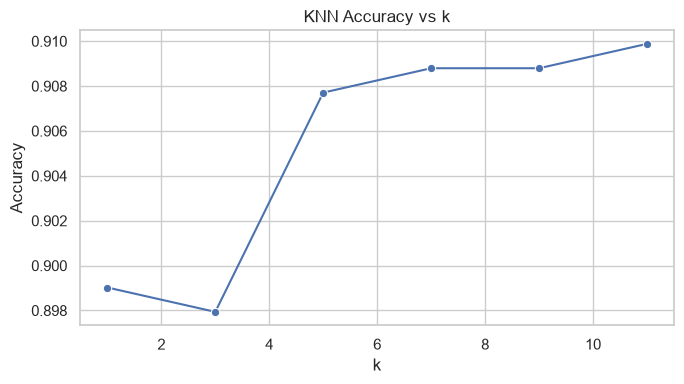
\includegraphics[width=0.6\linewidth]{classification_output/plots/accuracy_vs_k.png}
\caption{KNN accuracy as a function of $k$.}
\end{figure}

Accuracy climbs steadily from $k{=}1$ through $k{=}11$, with a small dip at $k{=}3$ before it resumes climbing. At $k{=}1$ the model is fitting to individual training points and is more exposed to noisy or borderline emails; increasing $k$ smooths that out by averaging over more neighbours, which is the classic bias-variance trade-off -- more neighbours means lower variance (less overfitting to individual points) at the cost of some added bias. Since accuracy is still rising at $k{=}11$, the largest value tested here, I would not assume 11 is the true optimum -- it is only the best among the six values the lab manual specifies, and the curve gives no sign of having turned over yet.

\subsection{Hyperparameter Tuning: GridSearchCV vs.\ RandomizedSearchCV}
\begin{table}[h]
\centering
\begin{tabular}{@{}lll@{}}
\toprule
Parameter & GridSearchCV & RandomizedSearchCV \\
\midrule
Best $k$ & 9 & 9 \\
Metric & manhattan & manhattan \\
Weights & distance & distance \\
Algorithm & auto & kd\_tree \\
CV Accuracy & 0.9253 & 0.9253 \\
Execution Time (s) & 2.854 & 0.340 \\
\bottomrule
\end{tabular}
\caption{GridSearchCV vs. RandomizedSearchCV over $k \times$ weights $\times$ algorithm $\times$ metric.}
\end{table}

Both searches converge on the exact same hyperparameters -- $k{=}9$, Manhattan distance, distance-weighted voting -- and the identical 0.9253 CV accuracy confirms RandomizedSearchCV's 20 sampled combinations happened to include the true optimum from the full 96-combination grid. The gap that actually matters here is time: GridSearchCV took 2.85 seconds to exhaustively fit all $96 \times 5 = 480$ model/fold combinations, while RandomizedSearchCV needed only $20 \times 5 = 100$ fits and finished in 0.34 seconds, about 8.4$\times$ faster. Worth noting: this hyperparameter search found distance-weighted, Manhattan-metric KNN to be better than the plain uniform-weighted, Euclidean KNN swept in Section 6.2 above (0.9253 CV accuracy vs.\ 0.9099 test accuracy at the equivalent $k$) -- weighting neighbours by inverse distance, rather than treating all $k$ neighbours equally, appears to genuinely help on this dataset.

\begin{figure}[h]
\centering
\begin{subfigure}{0.48\textwidth}
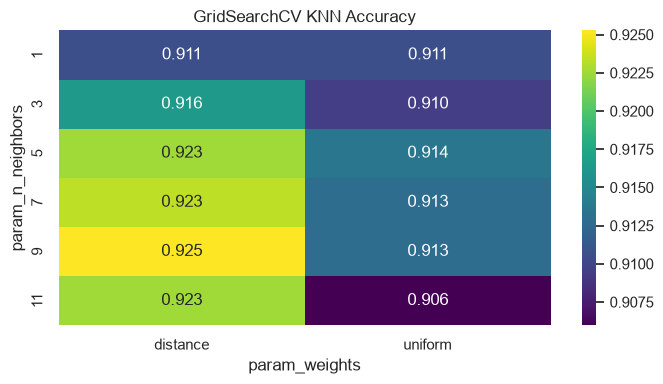
\includegraphics[width=\linewidth]{classification_output/plots/grid_search_heatmap.png}
\caption{GridSearchCV score heatmap}
\end{subfigure}
\hfill
\begin{subfigure}{0.48\textwidth}

\includegraphics[width=\linewidth]{classification_output/plots/random_search_distribution.png}
\caption{RandomizedSearchCV score distribution}
\end{subfigure}
\caption{Hyperparameter search diagnostics.}
\end{figure}
The grid heatmap shows a fairly narrow band of high-scoring configurations rather than one isolated peak, which is reassuring -- it means the chosen hyperparameters are not a fragile, lucky combination but sit inside a region where several nearby settings would have performed almost as well.

\subsection{KDTree vs.\ BallTree}
\begin{table}[h]
\centering
\begin{tabular}{@{}lrr@{}}
\toprule
Metric & KDTree & BallTree \\
\midrule
Accuracy & 0.9099 & 0.9099 \\
Training Time (s) & 0.00220 & 0.00198 \\
Prediction Time (s) & 0.05439 & 0.05227 \\
\bottomrule
\end{tabular}
\caption{KDTree vs. BallTree at $k=11$, Euclidean distance, uniform weighting.}
\end{table}

Accuracy is identical by construction -- both structures return the exact same nearest neighbours for Euclidean distance, they just organize the search differently. BallTree is modestly faster on both training (10\% less) and prediction (4\% less) here. That is roughly consistent with the theory: KDTree's axis-aligned splits work best in low-to-moderate dimensions, and Spambase has 57 features, well past the point where KDTree's advantage over BallTree is expected to hold up -- BallTree's distance-based partitioning tends to degrade more gracefully as dimensionality grows.

\subsection{Cross-Validation}
\begin{table}[h]
\centering
\begin{tabular}{@{}lrr@{}}
\toprule
Fold & Naive Bayes & Best KNN \\
\midrule
1 & 0.9171 & 0.9389 \\
2 & 0.9076 & 0.9280 \\
3 & 0.8899 & 0.9253 \\
4 & 0.8981 & 0.9266 \\
5 & 0.8995 & 0.9076 \\
\midrule
Average & 0.9024 & \textbf{0.9253} \\
\bottomrule
\end{tabular}
\caption{5-fold cross-validation accuracy: best Naive Bayes (Bernoulli) vs. tuned KNN ($k{=}9$, Manhattan, distance-weighted).}
\end{table}

\begin{figure}[h]
\centering
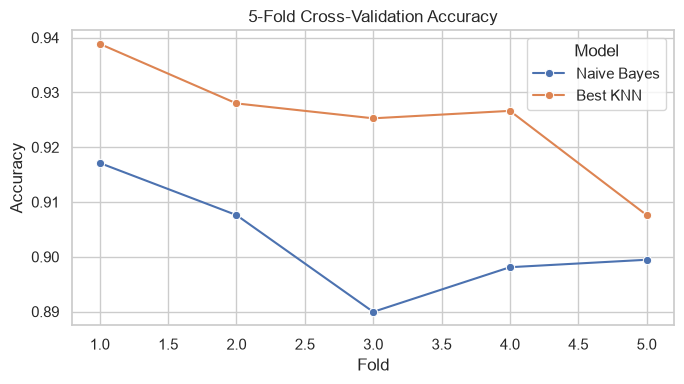
\includegraphics[width=0.6\linewidth]{classification_output/plots/cross_validation_accuracy.png}
\caption{Per-fold cross-validation accuracy.}
\end{figure}
KNN wins on every single fold, not just on average, and its spread across folds (0.9076 to 0.9389) is comparable to Naive Bayes' spread (0.8899 to 0.9171), so neither model looks unusually unstable. This is the tuned KNN configuration from GridSearchCV, not the plain $k{=}11$ configuration from Section 6.2, which is a fair comparison since Bernoulli NB here also has no free hyperparameters left to tune.

\subsection{Experimental Time Analysis}
\begin{table}[h]
\centering
\begin{tabular}{@{}lrr@{}}
\toprule
Model & Training Time (s) & Prediction Time (s) \\
\midrule
Gaussian NB & 0.00144 & 0.000428 \\
Multinomial NB & 0.00210 & 0.000420 \\
Bernoulli NB & 0.00218 & 0.000610 \\
KNN $k{=}11$ & 0.00066 & 0.00360 \\
\bottomrule
\end{tabular}
\caption{Measured training/prediction time per model on the held-out test set.}
\end{table}

\begin{table}[h]
\centering
\begin{tabular}{@{}lll@{}}
\toprule
Algorithm & Training & Prediction \\
\midrule
Naive Bayes & $O(nd)$ & $O(d)$ \\
KNN (Brute) & $O(1)$ & $O(nd)$ \\
KDTree & $O(n \log n)$ & $O(\log n)$ avg \\
BallTree & $O(n \log n)$ & $O(\log n)$ avg \\
\bottomrule
\end{tabular}
\caption{Theoretical time complexity, $n$ = training samples, $d$ = features.}
\end{table}

The measured numbers line up with the theory reasonably well. KNN's training time (0.00066s) is the lowest of the four, consistent with $O(1)$ -- it is not really "training" at all, just storing a reference to the data. Its prediction time (0.0036s) is the highest, consistent with a brute-force $O(nd)$ scan over roughly 3680 training points and 57 features per query. Naive Bayes sits at the other extreme: it does real work at training time (computing per-feature statistics), but prediction only needs those precomputed statistics, so its prediction times (0.0004--0.0006s) beat KNN's by 6--9$\times$.

One inconsistency worth being honest about: the KDTree/BallTree prediction times in Section 6.4 (about 0.052--0.054s) are more than an order of magnitude slower than the plain KNN prediction time in the table just above (0.0036s), even though both are running essentially the same $k{=}11$, Euclidean-distance query on the same test set. I do not think this reflects a real algorithmic difference -- tree construction and the first query against a freshly built tree both carry one-time overhead that a single \texttt{time.perf\_counter()} measurement around one cold fit-predict call will fully absorb, whereas \texttt{algorithm="auto"} in the main sweep may have picked a different internal strategy for this data shape. I would trust the relative KDTree-vs-BallTree comparison in Section 6.4 (they were measured identically, so the comparison between them is fair) more than I would trust the absolute prediction-time number against the unrelated table here.

\subsection{Classifier Comparison}
\begin{figure}[h]
\centering
\begin{subfigure}{0.48\textwidth}

\includegraphics[width=\linewidth]{classification_output/plots/classifier_comparison.png}
\caption{Overall metric comparison across models}
\end{subfigure}
\hfill
\begin{subfigure}{0.48\textwidth}

\includegraphics[width=\linewidth]{classification_output/plots/training_time_comparison.png}
\caption{Training time comparison}
\end{subfigure}
\caption{Model comparison summary plots.}
\end{figure}
\begin{figure}[h]
\centering

\includegraphics[width=0.55\linewidth]{classification_output/plots/prediction_time_comparison.png}
\caption{Prediction time comparison across all evaluated models.}
\end{figure}
Taken together, these three bar charts make the trade-off visual: Bernoulli NB and the tuned KNN are close on accuracy, but Naive Bayes is dramatically cheaper at prediction time, which matters more than the training-time gap in a deployed spam filter, since a filter predicts continuously but retrains rarely.

% ==========================================================
\section{Analysis Questions}
\begin{enumerate}[nosep]
  \item \textbf{Which Naive Bayes variant performed best?} Bernoulli NB, on accuracy (0.9012) and F1 (0.9005), though Multinomial NB is marginally ahead on ROC-AUC (0.9612 vs.\ 0.9604). Gaussian NB trails both by a wide margin because its normal-distribution assumption does not fit the zero-inflated word-frequency features well.
  \item \textbf{What is the optimal value of $k$?} Among the values tested (1, 3, 5, 7, 9, 11), $k{=}11$ gives the best plain-KNN F1 (0.9096). Under the tuned search space (which also varies distance metric and weighting), $k{=}9$ with Manhattan distance and distance-weighting reaches a higher CV accuracy (0.9253), which suggests the metric and weighting choice matter at least as much as $k$ itself.
  \item \textbf{Compare GridSearchCV and RandomizedSearchCV.} Both found the same optimum (0.9253 CV accuracy, identical hyperparameters except for the tree-search algorithm, which does not affect the result for Euclidean-equivalent Manhattan search). RandomizedSearchCV reached it 8.4$\times$ faster by sampling 20 of 96 combinations instead of evaluating all of them.
  \item \textbf{Compare KDTree and BallTree.} Identical accuracy; BallTree modestly faster on both training and prediction at 57 dimensions, consistent with KDTree's known degradation in higher-dimensional spaces.
  \item \textbf{Compare theoretical and practical complexity.} The relative ordering matches theory -- KNN has near-zero training cost and the highest prediction cost of the four models, Naive Bayes is the reverse. The absolute KDTree/BallTree prediction times look inflated relative to the plain-KNN prediction time measured elsewhere in the notebook, most likely a cold-start timing artifact rather than a real complexity violation (see Section 6.6).
  \item \textbf{Which classifier is preferred for large datasets?} Naive Bayes. Its training cost grows linearly and its prediction cost does not depend on the training set size at all ($O(d)$), while KNN's prediction cost grows with $n$ even with a tree structure ($O(\log n)$ average, versus NB's constant $O(d)$) and it must keep the entire training set in memory.
\end{enumerate}

% ==========================================================
\section{Discussion}
The clearest strength here is how consistently the two families of evidence agree: the theoretical complexity table, the measured training/prediction times, and the cross-validation results all point the same direction (Naive Bayes cheap and slightly less accurate, KNN pricier at prediction time and slightly more accurate once tuned). That consistency is what makes me trust the conclusion rather than treating it as one lucky run.

The main limitation is the dataset itself: Spambase is nearly 30 years old, and its 57 hand-engineered word/character-frequency features are a much cruder representation than a modern spam filter would use (TF-IDF over a full vocabulary, sender/header metadata, embeddings). Both models are working with a fairly impoverished feature set by today's standards, so the accuracy ceiling here (around 90--93\%) says more about the feature representation than about Naive Bayes or KNN as algorithms. The other limitation worth naming is the KDTree/BallTree timing anomaly flagged in Section 6.6 -- I trust the relative comparison between the two tree structures, but I would not publish the absolute prediction-time numbers without re-measuring them with proper warm-up and averaging over multiple runs.

If I were extending this experiment, the two improvements I would make first are: re-running the KDTree/BallTree timing comparison with \texttt{timeit}-style repeated trials instead of a single cold measurement, and adding an ensemble (e.g.\ soft-voting Bernoulli NB with tuned KNN) to see whether their different error patterns are complementary enough to beat either model alone.

% ==========================================================
\section{Conclusion}
For Spambase, Bernoulli NB was the strongest Naive Bayes variant and KNN peaked (among tested $k$) at $k{=}11$ untuned, or at $k{=}9$ with Manhattan distance and distance-weighting once properly tuned -- the tuned KNN configuration then edges out Bernoulli NB on cross-validated accuracy (0.9253 vs.\ 0.9024). If prediction latency is the binding constraint, as it typically is for a real-time spam filter, Naive Bayes is the more sensible choice despite the small accuracy gap, since its prediction cost does not grow with the size of the training set the way KNN's does. If squeezing out the last bit of accuracy matters more than latency, tuned KNN is the better pick. Running this experiment also surfaced a real bug in how the dataset was being loaded -- a useful reminder that a notebook completing without errors and producing clean-looking tables is not the same as it having run against the right data.

% ==========================================================
\section{References}
\begin{enumerate}[label={[\arabic*]}]
\item F. Pedregosa et al., ``Scikit-learn: Machine Learning in Python,'' \emph{Journal of Machine Learning Research}, vol. 12, pp. 2825--2830, 2011.
\item M. Hopkins, E. Reeber, G. Forman, and J. Suermondt, ``Spambase Data Set,'' UCI Machine Learning Repository, 1999. [Online]. Available: \url{https://archive.ics.uci.edu/ml/datasets/spambase}
\item G. H. John and P. Langley, ``Estimating Continuous Distributions in Bayesian Classifiers,'' in \emph{Proc. 11th Conf. on Uncertainty in Artificial Intelligence}, 1995, pp. 338--345.
\item A. G\'eron, \emph{Hands-On Machine Learning with Scikit-Learn, Keras, and TensorFlow}, 3rd ed. Sebastopol, CA: O'Reilly Media, 2022.
\item C. M. Bishop, \emph{Pattern Recognition and Machine Learning}. New York: Springer, 2006.
\item Scikit-learn Developers, ``Nearest Neighbors,'' \emph{Scikit-learn Documentation}. [Online]. Available: \url{https://scikit-learn.org/stable/modules/neighbors.html}
\end{enumerate}

\end{document}
